\documentclass{article} 
 \usepackage{trees}
 
\begin{document}
\title{Формула удаления и стягивания}
\author{Антон Петрунин}
\date{}
\maketitle


\section{Графы и их остовные деревья}

\begin{wrapfigure}{r}{32 mm}
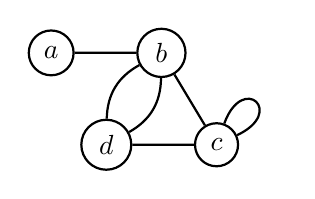
\begin{tikzpicture}[scale=1.4,
  thick,main node/.style={circle,draw,font=\sffamily\bfseries,minimum size=3mm}]

  \node[main node] (1) at (0,15/6) {$a$};
  \node[main node] (2) at (1,15/6){$b$};
  \node[main node] (11) at (1.5,10/6){$c$};
  \node[main node] (12) at (.5,10/6) {$d$};

  \path[every node/.style={font=\sffamily\small}]
   (11) edge [out=25,in=70,looseness=8] node[above] {} (11)
   (1) edge node{}(2)
   (2) edge[bend left] node{}(12)
   (2) edge[bend right] node{}(12)
   (2) edge node{}(11)
   (11) edge node{}(12)
   (12) edge node{}(12);
\end{tikzpicture}
\end{wrapfigure}

Рассмотрим план ежедневных рейсов некоторой авиакомпании между некоторыми парами из аэропортов $a,b,c$ и $d$
показанный не рисунке.
Для формализации такой и многих других ситуаций в математике используется понятие \emph{граф}.

Граф это конечный и не пустой набор \emph{вершин} (в нашем примере вершина графа это аэропорт) 
и конечный набор \emph{рёбер} каждое из которых соединяет пару вершин (в примере ребро это рейс авиакомпании).
Пара вершин графа может быть соединена несколькими рёбрами (это может означать, что авиакомпания совершает два рейса в день). 
Также, ребро может соединять вершину с самой собой, в этом случае оно называется \emph{петлёй} (про такое ребро можно думать как про прогулочный рейс авиакомпании).

То есть, с математической точки зрения, мы видим граф с четырьмя вершинами $a,b,c$ и $d$, 
шестью рёбрами, из них
одна петля при вершине $c$ и пара рёбер соединяет $b$ с $d$.
Число рёбер исходящих из данной вершины называется её \emph{степенью};
степени вершин $a,b,c$ и $d$ соответственно $1,4,4$ и~$3$.


Изображённый граф является \emph{связным}, то есть из любой его вершины можно пройти в любую другую пройдя по нескольким его рёбрам.

Предположим нам требуется сократить число рёбер связного графа сохранив его связность.
Нетрудно видеть, что это можно сделать тогда и только тогда, когда граф содержит \emph{цикл}.

Цикл это маршрут из рёбер обходящий несколько вершин без повторений вершин и рёбер 
и возвращается в исходную вершину. 
Число рёбер в цикле называется \emph{длиной цикла}.
Например в нашем графе есть два цикла  длины три с вершинами $b$, $c$ и $d$, 
один цикл длины два с вершинами $b$ и $d$,
a также петля при вершине $c$ образует цикл длины один.

Действительно, если из любого цикла связного графа выбросить любое ребро то граф останется связным.
Более того, если после выбрасывания некоторого ребра граф остался связным, то это ребро принадлежало некоторому циклу --- этот цикл образован самим ребром и кратчайшим путём между его концами в оствшемся графе.

Выбрасывание ребра из цикла можно повторять, пока мы не придём к графу без цикла.
Полученный граф называется остовным деревом исходного графа.

Вообще говоря, связный граф без циклов называется \emph{деревом}.
В~таких графах нет петель и из любой их вершины в любую другую есть единственный путь по рёбрам без повторений вершин.

На следующем рисунке вы видите все пять различных остовных дерева нашего исходного графа.

\label{page:5-derev}
\begin{center}
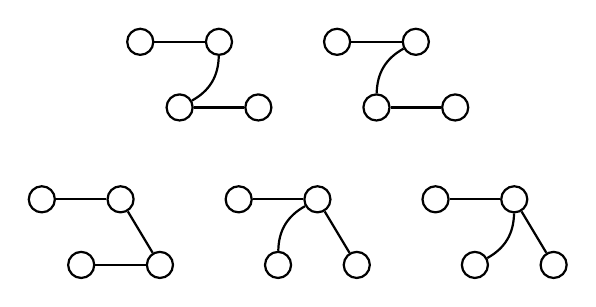
\begin{tikzpicture}[scale=1,
  thick,main node/.style={circle,draw,font=\sffamily\bfseries,minimum size=3mm}]

  \node[main node] (1) at (0,15/6) {};
  \node[main node] (2) at (1,15/6){};
  \node[main node] (11) at (1.5,10/6){};
  \node[main node] (12) at (.5,10/6) {};
  
  \node[main node] (101) at (0+2.5,15/6) {};
  \node[main node] (102) at (1+2.5,15/6){};
  \node[main node] (1011) at (1.5+2.5,10/6){};
  \node[main node] (1012) at (.5+2.5,10/6) {};
  
\node[main node] (201) at (0-1.25,15/6-2) {};
  \node[main node] (202) at (1-1.25,15/6-2){};
  \node[main node] (2011) at (1.5-1.25,10/6-2){};
  \node[main node] (2012) at (.5-1.25,10/6-2) {};
  
  \node[main node] (301) at (0+1.25,15/6-2) {};
  \node[main node] (302) at (1+1.25,15/6-2){};
  \node[main node] (3011) at (1.5+1.25,10/6-2){};
  \node[main node] (3012) at (.5+1.25,10/6-2) {};
  
   \node[main node] (401) at (0+3.75,15/6-2) {};
  \node[main node] (402) at (1+3.75,15/6-2){};
  \node[main node] (4011) at (1.5+3.75,10/6-2){};
  \node[main node] (4012) at (.5+3.75,10/6-2) {};
  
  \path[every node/.style={font=\sffamily\small}]
   (1) edge node{}(2)
   (2) edge[bend left] node{}(12)
   (11) edge node{}(12)
   
   
   (101) edge node{}(102)
   (102) edge[bend right] node{}(1012)
   (1011) edge node{}(1012)
  
   
   (201) edge node{}(202)
   (202) edge node{}(2011)
   (2011) edge node{}(2012)

   (301) edge node{}(302)
   (302) edge[bend right] node{}(3012)
   (302) edge node{}(3011)
   
   (401) edge node{}(402)
   (402) edge[bend left] node{}(4012)
   (402) edge node{}(4011);
\end{tikzpicture}
\end{center}


Чтобы проверить понимание данных определений мы советуем решить следующие два стандартных упражнения про деревья.

\begin{thm}{Упражнение}
Докажите что если дерево имеет хотябы две вершины, то в нём найдётся вершина степени 1.
\end{thm}


Воспользуйетесь индукцией по числу вершин и предыдущем упражнением чтобы доказать следующее.

\begin{thm}{Упражнение}
Докажите что число рёбер в любом дереве на один меньше числа его вершин.
\end{thm}


\section{Формула удаления и стягивания}

Пусть $\rho$ есть ребро в графе $\Gamma$.
Обозначим через $\Gamma\backslash\rho$ граф полученный из $\Gamma$ удалением ребра $\rho$
и через $\Gamma/\rho$ граф полученный из $\Gamma$ стягиванием ребра $\rho$ в точку.

Если ребро $\rho$ не является петлёй в $\Gamma$,  тогда выполняется следующее соотношение называемое \emph{формула удаления и стягивания}
\[\tau(\Gamma)=\tau(\Gamma\backslash\rho)+\tau(\Gamma/\rho).\leqno({*})\]

Действительно, остовные деревья в $\Gamma$ можно разделить на две категории ---
те что содержат ребро $\rho$ и те, что его не содержат.
Для деревьев из первой категории стягивание ребра $\rho$ в точку даёт остовое дерево в $\Gamma/\rho$ а деревья второй категории являются также остовными деревьями в графе  $\Gamma\backslash\rho$.
Более того, оба этих соответствия взаимно однозначны.
Отсюда вытекает формула.

Например, если $\Gamma$ это первый пример и $\rho$ есть ребро между вершинами $b$ и $c$,
тогда первые два остовных дерева на странице \pageref{page:5-derev} соответсвуют дереву в $\Gamma\backslash\rho$, а последние два соответствуют дереву в $\Gamma/\rho$.

\begin{wrapfigure}{r}{40 mm}
\begin{lpic}[t(0 mm),b(0 mm),r(0 mm),l(0 mm)]{pics/osnovnoe-ravenstvo(1)}
\lbl[tr]{4,10;$\Gamma$}
\lbl[br]{28,26;$\Gamma\backslash\rho$}
\lbl[tr]{28,5;$\Gamma/\rho$}
\end{lpic}
\end{wrapfigure}

Формулу удаления и стягивания $({*})$ удобно записывать схематически как показано на рисунке.
На графе $\Gamma$ ребро $\rho$ для которого применяется формула отмечено одним штрихом. 

Заметим, что никакое остовое дерево не содержит петель.
Поэтому можно выбросить все петли из графа и число его остовных деревьев останется неизменным.
Иначе говоря, для любой петли $\rho$ выполняется равенство 
\[\tau(\Gamma)=\tau(\Gamma\backslash\rho).\]

Из формулы удаления и стягивания можно вывести несколько других полезных соотношений.
Например если в графе $\Gamma$ есть вершина $w$ степени 1 то $w$ и ребро при $w$ можно 
выбросить из графа и в полученном графе $\Gamma\backslash w$ число его остовных графов не изменится, то есть
\[\tau(\Gamma)=\tau(\Gamma\backslash w).\]
Действительно, обозначим через $\rho$ единственное ребро при $w$. 
Заметим, что граф $\Gamma\backslash\rho$ не связен, поскольку вершина $w$ не имеет рёбер, и значит 
$\tau(\Gamma\backslash\rho)=0$.
С другой стороны $\Gamma/\rho=\Gamma\backslash w$, отсюда получаем равенство.

На схемах двусторонняя стралка ``$\leftrightarrow$'' будет означать, что соотвветсвующие графы имеют то же число остовных деревьев, например из выведенных тождеств можно вывести следующую диаграмму 
\begin{center}
\begin{lpic}[t(0 mm),b(0 mm),r(0 mm),l(0 mm)]{pics/diagramma(1)}
\lbl[tr]{3,15;$\Gamma$}
\lbl[tl]{54,15;$\Delta$}
\end{lpic}
\end{center}
означающую в частности, что $\tau(\Gamma)=2\cdot\tau(\Delta)$.

Равенства описанные выше дают алгоритм вычисления $\tau(\Gamma)$.
Действительно, для любого ребра $\rho$, оба графа $\Gamma\backslash\rho$ и $\Gamma/\rho$ имеют меньшее число рёбер.
То есть формула удаления и стягивания сводит нахождение числа остовных деревьев $\Gamma$ к нахождению числа остовных деревьев \emph{более простых} графов.


\medskip

\begin{wrapfigure}[4]{r}{42 mm}
\begin{lpic}[t(-7 mm),b(0 mm),r(0 mm),l(0 mm)]{pics/most(1)}
\lbl[b]{21,8;мост}
\lbl[t]{7,0;остров}
\lbl[t]{34,0;остров}
\end{lpic}
\end{wrapfigure}

В заключении ещё одно упражнение.
Ребро связного графа называется \emph{мостом} если удаление этого ребра из графа делает граф не свазным,
такой граф разбивается на два связных графа называемыми его \emph{островами}.

\begin{thm}{Упражнение}
Предположим граф $\Gamma$ содержит мост между островами $\Delta_1$ и $\Delta_2$.
Докажите, что
\[\tau(\Gamma)=\tau(\Delta_1)\cdot\tau(\Delta_2).\]
\end{thm}
 
\section{Деревья в веерах}

Графы следующего вида называются \emph{веерами}; 
веер с $n+1$ вершиной будет обозначаться $\Theta_n$. 

\begin{center}
\begin{lpic}[t(0 mm),b(0 mm),r(0 mm),l(-10 mm)]{pics/veera(1)}
\lbl[br]{12,15;$\Theta_1$}
\lbl[br]{27.5,16.5;$\Theta_2$}
\lbl[br]{43.2,17.5;$\Theta_3$}
\lbl[br]{57.5,18.5;$\Theta_4$}
\lbl[br]{73,20;$\Theta_5$}
\lbl[l]{83,14;{\Large$\dots$}}
\end{lpic}
\end{center}

Применив соотношения полученные выше можно составить следующую бесконечную схему.
В дополнении к веерам, $\Theta_n$ в схеме участвуют их вариации $\Theta_n'$, отличающиеся от $\Theta_n$ дополнительным ребром.
\begin{center}
\begin{lpic}[t(0 mm),b(0 mm),r(0 mm),l(0 mm)]{pics/veera-skhema(1)}
\lbl[br]{4,49;$\Theta_6$}
\lbl[br]{42,49;$\Theta_5$}
\lbl[br]{76,47;$\Theta_4$}
\lbl[tr]{25,7;$\Theta'_5$}
\lbl[tr]{63,8;$\Theta'_4$}
\lbl[l]{77,13;{\Large$\dots$}}
\lbl[r]{17,13;{\Large$\dots$}}
\lbl[r]{0,43;{\Large$\dots$}}
\lbl[l]{85,43;{\Large$\dots$}}
\end{lpic}
\end{center}

Введём обозначения $a_n=\tau(\Theta_n)$ и $a'_n=\tau(\Theta'_n)$.
Из схемы легко вывести два рекуррентных соотношения:
\begin{align*}
a_{n+1}&=a'_n+a_n,
\\
a'_n&=a_n+a'_{n-1}.
\end{align*}
То есть в последоватльности чисел
\[a_1,a_1',a_2,a_2',a_3\dots\]
каждое следующее является суммой двух предыдущих.

Напомним, что последовательность чисел Фибоначи $F_n$ задаётся тем же соотношением 
$F_{n+1}=F_n+F_{n-1}$ с $F_1=F_2=1$.
Она начинается следующим образом
\[1,1,2,3,5,8,13,\dots\]

Далее заметим, что $\Theta_1$ это две вершины соединённые единственным ребером,
а $\Theta'_1$ это две вершины соединённые двойным ребром.
Отсюда $a_1=1=F_2$ и $a_1'=2=F_3$ и значит 
\[a_n=F_{2\cdot n}\]
для любого $n$.

Можно также вывести соотношение на $a_n$, без $a_n'$:
\begin{align*}
a_{n+1}&=a_n'+a_n=
\\
&=2\cdot a_n+a'_{n-1}=
\\
&=3\cdot a_n-a_{n-1}.
\end{align*}

Оказывается, что если последовательность задаётся подобным соотношением
то можно найти формулу для её общего члена.
В нашем случае \[a_n=\tfrac1{\sqrt{5}}\cdot
\left(
(\tfrac{3+\sqrt{5}}2)^n-(\tfrac{3-\sqrt{5}}2)^n
\right).\]
Этот процесс подробно описан в книжке \cite{markushevich}, которую мы рекомендуем читателю.

\medskip

Для закрепления материала мы советуем разобрать следующую задачу.

Пусть $b_n$ обозначает число остовных деревьев в \emph{лестнице} $\Lambda_n$ с $n$ ступеньками, то есть в графе следующего типа.

\begin{center}
\begin{lpic}[t(0 mm),b(0 mm),r(0 mm),l(0 mm)]{pics/a1-4(1)}
\lbl[b]{5.5,4;$\Lambda_1$}
\lbl[b]{15.5,9;$\Lambda_2$}
\lbl[b]{25.5,14;$\Lambda_3$}
\lbl[b]{35.5,19;$\Lambda_4$}
\lbl[b]{45.5,24;$\Lambda_5$}
\lbl[l]{50.5,13;{\Large$\dots$}}
\end{lpic}
\end{center}

Воспользуйтесь разработанным методом и докажите, что последовательность $b_n$ удовлетворяет следующему рекуррентному соотношению 
\[b_{n+1}=4\cdot b_n-b_{n-1}.\]

\begin{wrapfigure}{r}{20 mm}
\begin{lpic}[t(-10 mm),b(0 mm),r(0 mm),l(0 mm)]{pics/lestnitza-shtrih(1)}
\lbl[b]{5,23.5;$\Lambda_3'$}
\lbl[b]{15,21;$\Lambda_3''$}
\end{lpic}
\end{wrapfigure}

Заметим, что $b_1=1$ и $b_2=4$ отсюда можно быстро посчитать первые члены последовательности:
\[1,4,15,56,209,780,2911,\dots \]

Вам потребуются ещё пара последовательностей графов, 
$\Lambda_n'$ и $\Lambda_n''$ показанных на рисунке.

\medskip

Если упражнение выше показалось слишком легким, сделайте тоже для колёс;
то есть графов $\Phi_n$ следующего типа.
\begin{center}
\begin{lpic}[t(1 mm),b(0 mm),r(0 mm),l(0 mm)]{pics/kolesa(1)}
\lbl[br]{3,11;$\Phi_1$}
\lbl[b]{16,11;$\Phi_2$}
\lbl[b]{30.5,11;$\Phi_3$}
\lbl[b]{46,11;$\Phi_4$}
\lbl[b]{61.5,11;$\Phi_5$}
\lbl[l]{74,7;{\Large$\dots$}}
\end{lpic}
\end{center}
Для  $c_n=\tau(\Phi_n)$ правильный ответ
\[c_{n+1}=4\cdot c_n-4\cdot c_{n-1}+c_{n-2}.\]



\section{Графы как матрицы}

{

\begin{wrapfigure}{r}{32 mm}
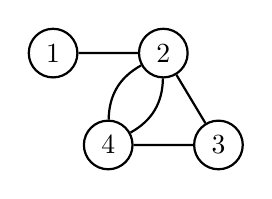
\begin{tikzpicture}[scale=1.4,
  thick,main node/.style={circle,draw,font=\sffamily\bfseries,minimum size=3mm}]

  \node[main node] (1) at (0,15/6) {$1$};
  \node[main node] (2) at (1,15/6){$2$};
  \node[main node] (11) at (1.5,10/6){$3$};
  \node[main node] (12) at (.5,10/6) {$4$};

  \path[every node/.style={font=\sffamily\small}]
  
   (1) edge node{}(2)
   (2) edge[bend left] node{}(12)
   (2) edge[bend right] node{}(12)
   (2) edge node{}(11)
   (11) edge node{}(12)
   (12) edge node{}(12);
\end{tikzpicture}
\end{wrapfigure}

Предположим вершины графа $\Gamma$ пронумерованы числами от $1$ до $n$.
Тогда граф $\Gamma$ можно полностью описать таблицей $n\times n$ поставив в клетки на пересечении $i$-ой строки и $j$-ого столбца число рёбер соединяющих $i$-ую вершину графа с и $j$-ой.

}

Полученная таблица $A=A_\Gamma$ называется \emph{матрицей смежности графа}.
Она симметрична, то есть отражение в главной диагонали переставляет равные числа.
Для графа на рисунке получим 

\[A=\left(
\begin{matrix}
0&1&0&0
\\
1&0&1&2
\\
0&1&0&1
\\
0&2&1&0
\end{matrix}
\right)\]

Поскольку наличие петель не влияет на число остовных деревьев, мы можем считать, что граф не содержит петель.
В этом случае на главной диагонали $A$ стоят нули.

Поскольку матрица смежности полностью описывает исходный граф, 
число остовных деревьев графа в принципе можно вычислить по его матрице смежностей.

Оказывается, это довольно легко сделать.
Сначала из построенной $n\times n$-матрицы  $A$ нашего графа $\Gamma$ нужно построить $(n-1)\times(n-1)$-матрицу $K$ следующим образом: 

\begin{enumerate}
\item Обратим знаки всех компонент матрицы $A$ и заменим нули на её диагонали степенями соответствующих вершин. 
В полученной матрице $A'$ сумма чисел в каждой строке и в каждом столбце равна нулю. 
\item Выбросим из матрицы $A'$ последнюю строку и последний столбец;
обозначим через $K=K_\Gamma$ полученную матрицу.
\end{enumerate}

Для нашего примера имеем

\[A'=\left(
\begin{matrix}
1&-1&0&0
\\
-1&4&-1&-2
\\
0&-1&2&-1
\\
0&-2&-1&3
\end{matrix}
\right),
\quad 
K=\left(
\begin{matrix}
1&-1&0
\\
-1&4&-1
\\
0&-1&2
\end{matrix}
\right)\]

По матрице $K$ можно восстановить $A'$, а значит и матрицу $A$ и граф $\Gamma$ если у него не было петель.
Действительно, чтобы получить $A'$ нужно добавить строку и столбец к матрице $K$ и заполнить их числами так, чтобы сумма в каждой строке и столбце была нулевой;
это можно сделать единственным образом.

Таким образом по матрице $K$ можно найти число $\delta(K)$ равное $\tau(\Gamma)$, то есть числу деревьев исходного графа.
Для $\delta(K)$ верны следующие соотношения:
\begin{enumerate}
\item Eсли в матрице $K$ поменять местами пару строк и пару столбцов с теми же номерами,
тогда для полученной матрицы $K'$ выполняется 
\[\delta(K)=\delta(K').\]
Действительно, $K'$ описывать тот же граф $\Gamma$ с другой нумерацией вершин.
\item 
Если сумма компонент первой строки в $K$ положительна, то
\[\delta(K)=\delta(K^{\circ})+\delta(K^{\bullet})\]
где $K^{\circ}$ обозначает матрицу $K$ в которой от углового компоненты отняли 1, а $K^{\bullet}$ обозначает $(n-2)\times(n-2)$ матрицу полученную из $K$ удалением первого столбца и первой строки.
Это равенство следует из формулы удаления и стягивания $({*})$ поскольку \[K^{\circ}=K_{\Gamma\backslash\rho}\quad\text{и}\quad K^{\bullet}=K_{\Gamma/\rho}.\]
\item Если сумма чисел в каждой строке $K$ равна $0$ то $\delta(K)=0$. 
Действительно, в этом случае ни одна из вершин исходного графа не связана с последней вершиной, а значит граф несвязен и не имеет остовных деревьев.
\end{enumerate}

Читатель знакомый с понятием определитель%
\footnote{Для читателей незнакомых с понятием определитель написана следующая главка.}
непременно заметит, что
тем же свойствам обладает и \emph{определитель матрицы} $K$ далее обозначаемый $|K|$.
Поскольку эти свойства полностью определяют $\delta(K)$ мы получаем 
\[\delta(K)=| K|.\]


Отсюда следует так называемая матричная формула Кигхофа
\[\tau(\Gamma)=| K_\Gamma|.\leqno({*}{*})\]

Идея доказательства поучительна ---  равенство двух разношёрстно определённых числа
$\tau(\Gamma)$ и $|K_\Gamma|$ следует из общих свойств этих чисел. 
Эту идею можно рассматривать как обобщение метода математической индукции;
она имеет множество других приложений, но к сожалению более простые содержательные примеры нам не известны.


\section{Ликбез на тему «определители»}

\emph{Квадратная матрица} это таблица $n{\times}n$ заполненная числами называемыми её \emph{компонентами}.
Определитель $| M|$ матрицы $M$ это многочлен от её $n^2$ её компонент,
который удовлетворяет следующим условиям:
\begin{enumerate}
 \item\label{1} Определитель единичной матрицы равен 1; то есть,
\[
\left|
\begin{matrix}
1&0&\cdots&0
\\
0&1&\ddots&\vdots
\\
\vdots&\ddots&\ddots&0
\\
0&\cdots&0&1
\end{matrix}
\right|=1.
\]
\item\label{2} Если каждую компоненту одной из строк матрицы $M$ умножить на число $\lambda$ то определитель полученной матрицы $M'$ умножится на то же число, то есть
\[|M'|=\lambda\cdot |M|.\]
\item\label{3} Если одну из строк матрицы $M$ почленно прибавить к другой строке (или отнять от неё) то определитель полученной матрицы $M'$ не изменится, то есть
\[|M'|= |M|.\]
\end{enumerate}

Вышеприведённые свойства однозначно определяют определитель.
Мы примем это утверждение без доказательства; оно неочевидное, но и несложное, 
кроме того рано или поздно вам придётся его выучить.

\begin{thm}{Упражнение}
Выведите следующее свойство из трёх перечисленных выше.
\end{thm}

\begin{enumerate}[resume]
 \item 
Если две строки матрицы $M$ поменять местами то определитель полученной матрицы $M'$ поменяет знак; то есть,
\[|M'|=-|M|.\]
\end{enumerate}


Для определителя можно выписать явную формулу из $n!$ слагаемых
однако свойства определителя описанные выше дают более удобный и быстрый способ вычисления определителя.

Мы разберём этот способ на одном примере, который нам пригодится позже:
\begin{align*}
&\left|
\begin{matrix}
4&-1&-1&-1
\\
-1&4&-1&-1
\\
-1&-1&4&-1
\\
-1&-1&-1&4
\end{matrix}
\right|
=
\left|
\begin{matrix}
1&1&1&1
\\
-1&4&-1&-1
\\
-1&-1&4&-1
\\
-1&-1&-1&4
\end{matrix}
\right|=
\intertext{Первое равенство следует из свойства \ref{3}; мы по очереди прибавили к первой строке все строки со второй до последней. Далее мы прибавили первую ко всем остальным, и применили свойство \ref{2} три раза:}
&=\left|
\begin{matrix}
1&1&1&1
\\
0&5&0&0
\\
0&0&5&0
\\
0&0&0&5
\end{matrix}
\right|
=
5^3\cdot
\left|
\begin{matrix}
1&1&1&1
\\
0&1&0&0
\\
0&0&1&0
\\
0&0&0&1
\end{matrix}
\right|=
\intertext{отняв от первой строки все остальные строки, и применив свойства \ref{1}, получаем}
&=
5^3\cdot\left|
\begin{matrix}
1&0&0&0
\\
0&1&0&0
\\
0&0&1&0
\\
0&0&0&1
\end{matrix}
\right|
=5^3.
\end{align*}


\section{Формула Кэли}

Прямое обобщение вычисления данного выше даёт, что
\[|K|=n^{n-2},\]
где $K$ обозначает $(n-1)\times (n-1)$ матрицу следующего вида:
\[
K=\left(
\begin{matrix}
n{-}1&-1&\cdots&-1
\\
-1&n{-}1&\ddots&\vdots
\\
\vdots&\ddots&\ddots&-1
\\
-1&\cdots&-1&n{-}1
\end{matrix}
\right)
\]
Матрица $K$ это как раз матрица в матричной формуле $({*}{*})$ для полного графа $\Pi_n$ с $n$ вершинами.
\emph{Полным графом} называется граф в котором любая пара различных вершин соединена единственным ребром; то есть, получаем 
\[\tau(\Pi_n)=n^{n-2}.\]
Это равенство называется \emph{формулой Кэли}.


\section{Замечания}

\emph{Формула удаления и стягивания} применялясь при решении так называемой \emph{задачи о квадрировании квадрата}.
История этой задачи и её замечательное решение обсудаются в книжках \cite{yaglom} и \cite[Глава 32]{gardner}.
Близкое тождество выполняется для \emph{хроматического многочлена}
\[P(\Gamma,t)=P(\Gamma\backslash\rho,t)-P(\Gamma/\rho,t),\] 
то есть $P(\Gamma,t)$ обозначает число раскрасок графа $\Gamma$ в $t$ цветов такое, что концы каждого ребра покрашены в разные цвета.

Приведённый нами вывод рекуррентных формул для чисел остовных деревьев в веерах лестницах и колёсах даётся в \cite{haghighi-bibak}.

Матричное тождество $({*}{*})$ было открыто Густавом Кирхгофом в  1847 году при изучении свойств электрических цепей с использованием правил известными сейчас как \emph{правила Кирхгофа}.
Есть множество других приложений правил Киргхофа в теории графов. 
Например оно используется в физическом доказательстве формулы Эйлера
\[\text{В}-\text{Р}+\text{Г}=2,\]
где $\text{В}$, $\text{Р}$ и $\text{Г}$ обозначает число вершин, рёбер и граней многогранника,
смотри \cite{levi}.  

Несколько красивых доказательств формулы Кэли и её история осуждаются в \cite[Глава 30]{aigner-ziegler}.

\begin{thebibliography}{52}
\bibitem{markushevich}
А. И. Маркушевич,
\emph{Возвратные последовательности,} 
Гостехиздат, 1950. (Популярные лекции по математике, вып. 1.).

\bibitem{aigner-ziegler} М. Айгнер, Г. Циглер, 
\emph{Доказательства из Книги,} 
Бином. Лаборатория знаний, 2015 

\bibitem{gardner} М. Гарднер, \emph{Математические головоломки и развлечения,}  Оникс, Москва, 1994.

\bibitem{yaglom}
И. М. Яглом,
\emph{Как разрезать квадрат?}
М., Наука, 1968.

\bibitem{levi} M. Levi,
An Electrician’s (or a Plumber’s)
Proof of Euler’s Polyhedral Formula,
\emph{SIAM News} 50, no. 4, May 2017


\bibitem{haghighi-bibak} M. H. Shirdareh Haghighi; Kh. Bibak, 
Recursive relations for the number of spanning trees. 
\emph{Appl. Math. Sci. (Ruse)} 3 (2009), no. 45--48, 2263--2269. 
\end{thebibliography}



\end{document}

\section{Общая формула}

Сначала следует найти геометрические прогрессии $a_n=c\cdot \lambda^n$ удовлетворяющие нашему рекуррентному соотношению $({*}{*})$.
То есть значения $c$ и $\lambda$ такие, что
\[c\cdot\lambda^{n+1}=3\cdot c\cdot\lambda^n-c\cdot\lambda^{n-1}.\]
При $c\ne0$, это уравнение сводится к квадратному уравнению на $\lambda$
\[\lambda^2-3\cdot\lambda+1=0;\]
оно имеет два решения $\lambda_1=\tfrac{3+\sqrt{5}}2$ и $\lambda_2=\tfrac{3-\sqrt{5}}2$.

Заметим, что для любых $c_1$ и $c_2$ последовательности $c_1\cdot\lambda_1^n$ и $c_2\cdot\lambda_2^n$, а значит и их сумма $a_n=c_1\cdot\lambda_1^n+c_2\cdot\lambda_2^n$ удолетворёют рекурсивному соотношению $({*}{*})$.
Остаётся подобрать константы $c_1$ и $c_2$ такие, что $a_0=1$ и $a_1=5$, то есть решить систему уравнений
$$
\left[
\begin{aligned}
c_1\cdot \tfrac{3+\sqrt{5}}2+c_2\cdot \tfrac{3-\sqrt{5}}2=1,
\\
c_1\cdot (\tfrac{3+\sqrt{5}}2)^2+c_2\cdot (\tfrac{3-\sqrt{5}}2)^2=5.
\end{aligned}
\right.
$$
Мы получаем следующую формулу для общего члена:
\[a_n=\tfrac1{\sqrt{5}}\cdot\left((\tfrac{3+\sqrt{5}}2)^n-(\tfrac{3-\sqrt{5}}2)^n\right).\]

Заметим, что второе слагаемое в формуле отрицательно и меньше $1$ по абсолютной величине.
Поскольку $a_n$ целое, получаем
\[a_n=\left\lceil\tfrac1{\sqrt{5}}\cdot(\tfrac{3+\sqrt{5}}2)^n\right\rceil,\]
где $\lceil x\rceil$ обозначает наименьшее целое число не меньшее $x$. 

Для полученного рекуррентного соотношения выведите формулы общего члена
\begin{align*}
b_n
&=
\tfrac1{2\cdot\sqrt{3}}\cdot\left((2+\sqrt{3})^n+(2-\sqrt{3})^n\right)
\intertext{и}
b_n&=\left\lceil\tfrac1{2\cdot\sqrt{3}}\cdot(2+\sqrt{3})^n\right\rceil.
\end{align*}
